%% LLT: Turn off some annoying warnings...
\RequirePackage{silence}
\WarningFilter{titlesec}{Non standard sectioning command}
\WarningFilter{scrreprt}{Usage of package}
\WarningFilter{scrreprt}{Activating an ugly workaround}
% **************************************************
% Document Class Definition
% **************************************************
\documentclass[%
	paper=A4,
	twoside=true,				% onesite or twoside printing
	openright,					% doublepage cleaning ends up right side
	parskip=full,				% spacing value / method for paragraphs
	chapterprefix=true,			% prefix for chapter marks
	11pt,						% font size
	headings=normal,			% size of headings
	bibliography=totoc,			% include bib in toc
	listof=totoc,				% include listof entries in toc
	titlepage=on,				% own page for each title page
	captions=tableabove,		% display table captions above the float env
	draft=false,				% value for draft version
]{scrreprt}
\usepackage[utf8]{inputenc}

% **************************************************
% Debug LaTeX Information
% **************************************************
%\listfiles

% **************************************************
% Information and Commands for Reuse
% **************************************************
\newcommand{\thesisTitle}{Deep Learning Next Event Prediction With Subsequence-Enrichted Input Data}
\newcommand{\thesisName}{Felix Wolff}
\newcommand{\thesisSubject}{Master's thesis}
\newcommand{\thesisDate}{February 20, 2019}
\newcommand{\thesisVersion}{My First Draft}

\newcommand{\thesisFirstReviewer}{Prof. Dr. Mathias Weske}
\newcommand{\thesisFirstReviewerUniversity}{\protect{Hasso Plattner Institut}}
\newcommand{\thesisFirstReviewerDepartment}{Business Process Technology Group}

\newcommand{\thesisSecondReviewer}{Prof. Dr. ????????????}
\newcommand{\thesisSecondReviewerUniversity}{\protect{????????????}}
\newcommand{\thesisSecondReviewerDepartment}{????????????}

\newcommand{\thesisFirstSupervisor}{Dr. Luise Pufahl}
\newcommand{\thesisSecondSupervisor}{Dr. Haojin Yang}

\newcommand{\thesisUniversity}{\protect{Hasso Plattner Institut}}
\newcommand{\thesisUniversityDepartment}{Business Process Technology Group}
\newcommand{\thesisUniversityInstitute}{}
\newcommand{\thesisUniversityGroup}{}
\newcommand{\thesisUniversityCity}{Potsdam}
\newcommand{\thesisUniversityStreetAddress}{Prof.-Dr.-Helmert-Straße 2-3}
\newcommand{\thesisUniversityPostalCode}{14482}

% **************************************************
% Load and Configure Packages
% **************************************************
\usepackage[english]{babel}
\usepackage[
	figuresep=colon,%
	sansserif=false,%
	hangfigurecaption=false,%
	hangsection=true,%
	hangsubsection=true,%
	colorize=full,%
	colortheme=bluemagenta,
	bibsys=biber,%
	bibfile=bib-refs,%
	bibstyle=numeric,
]{cleanthesis}

\hypersetup{					% setup the hyperref-package options
	pdftitle={\thesisTitle},	% 	- title (PDF meta)
	pdfsubject={\thesisSubject},% 	- subject (PDF meta)
	pdfauthor={\thesisName},	% 	- author (PDF meta)
	plainpages=false,			% 	-
	colorlinks=false,			% 	- colorize links?
	pdfborder={0 0 0},			% 	-
	breaklinks=true,			% 	- allow line break inside links
	bookmarksnumbered=true,		%
	bookmarksopen=true			%
}
\usepackage{todonotes}

% **************************************************
% Document CONTENT
% **************************************************
\begin{document}

% --------------------------
% rename document parts
% --------------------------
%\renewcaptionname{ngerman}{\figurename}{Abb.}
%\renewcaptionname{ngerman}{\tablename}{Tab.}
%\renewcaptionname{english}{\figurename}{Fig.}
%\renewcaptionname{english}{\tablename}{Tab.}

% --------------------------
% Front matter
% --------------------------
\pagenumbering{roman}			% roman page numbing (invisible for empty page style)
\pagestyle{empty}				% no header or footers
% ------------------------------------  --> cover title page
\begin{titlepage}
	\pdfbookmark[0]{Cover}{Cover}
	\flushright
	\hfill
	\vfill
	{\LARGE\thesisTitle \par}
	\rule[5pt]{\textwidth}{.4pt} \par
	{\Large\thesisName}
	\vfill
	\textit{\large\thesisDate} \\
	Version: \thesisVersion
\end{titlepage}


% ------------------------------------  --> main title page
\begin{titlepage}
	\pdfbookmark[0]{Titlepage}{Titlepage}
	\tgherosfont
	\centering

	%{\Large \thesisUniversity} \\[4mm]
	
\includegraphics[width=6cm]{gfx/hpi_logo} \\[2mm]
	\textsf{\thesisUniversityDepartment} \\
	\textsf{\thesisUniversityInstitute} \\
	\textsf{\thesisUniversityGroup} \\

	\vfill
	{\large \thesisSubject} \\[5mm]
	{\LARGE \color{ctcolortitle}\textbf{\thesisTitle} \\[10mm]}
	{\Large \thesisName} \\

	\vfill
	\begin{minipage}[t]{.27\textwidth}
		\raggedleft
		\textit{1. Reviewer}
	\end{minipage}
	\hspace*{15pt}
	\begin{minipage}[t]{.65\textwidth}
		{\Large \thesisFirstReviewer} \\
	  	{\small \thesisFirstReviewerDepartment} \\[-1mm]
		{\small \thesisFirstReviewerUniversity}
	\end{minipage} \\[5mm]
	\begin{minipage}[t]{.27\textwidth}
		\raggedleft
		\textit{2. Reviewer}
	\end{minipage}
	\hspace*{15pt}
	\begin{minipage}[t]{.65\textwidth}
		{\Large \thesisSecondReviewer} \\
	  	{\small \thesisSecondReviewerDepartment} \\[-1mm]
		{\small \thesisSecondReviewerUniversity}
	\end{minipage} \\[10mm]
	\begin{minipage}[t]{.27\textwidth}
		\raggedleft
		\textit{Supervisors}
	\end{minipage}
	\hspace*{15pt}
	\begin{minipage}[t]{.65\textwidth}
		\thesisFirstSupervisor\ and \thesisSecondSupervisor
	\end{minipage} \\[10mm]

	\thesisDate \\

\end{titlepage}


% ------------------------------------  --> lower title back for single page layout
\hfill
\vfill
{
	\small
	\textbf{\thesisName} \\
	\textit{\thesisTitle} \\
	\thesisSubject, \thesisDate \\
	Reviewers: \thesisFirstReviewer\ and \thesisSecondReviewer \\
	Supervisors: \thesisFirstSupervisor\ and \thesisSecondSupervisor\\[1.5em]
	\textbf{\thesisUniversity} \\
	\textit{\thesisUniversityGroup} \\
	\thesisUniversityInstitute \\
	\thesisUniversityDepartment \\
	\thesisUniversityStreetAddress \\
	\thesisUniversityPostalCode\ and \thesisUniversityCity
}
		% INCLUDE: all titlepages
\cleardoublepage

\pagestyle{plain}				% display just page numbers
% !TEX root = ../thesis-example.tex
%
\pdfbookmark[0]{Abstract}{Abstract}
\chapter*{Abstract}
\label{sec:abstract}
\vspace*{-10mm}


\vspace*{20mm}

{\usekomafont{chapter}Abstract (German)}\label{sec:abstract-german} \\

Is this really needed?!		% INCLUDE: the abstracts (english and german)
\cleardoublepage
%
% !TEX root = ../thesis-example.tex
%
\pdfbookmark[0]{Acknowledgement}{Acknowledgement}
\chapter*{Acknowledgement}
\label{sec:acknowledgement}
\vspace*{-10mm}

Luise Pufahl
Haojin Yang
Feng Cheng
Willi Gierke (LSTM questions) % INCLUDE: acknowledgement
\cleardoublepage
%
\setcounter{tocdepth}{2}		% define depth of toc
\tableofcontents				% display table of contents
\cleardoublepage

% --------------------------
% Body matter
% --------------------------
\pagenumbering{arabic}			% arabic page numbering
\setcounter{page}{1}			% set page counter
\pagestyle{maincontentstyle} 	% fancy header and footer

\chapter{Introduction}\label{sec:intro}

\cleanchapterquote{The most important contribution of management in the 20th century was to increase manual worker productivity fifty-fold. The most important contribution of management in the 21st century will be to increase knowledge worker productivity—hopefully by the same percentage.}{Peter Drucker}{(American management consultant and professor)}

\section{Research questions}\label{sec:intro:objective}
In my thesis, I want to investigate the synergies of combining the aforementioned approach of Francescomarino et al. for learning data clustering with LSTM neural networks as per Evermann et al. Case data attributes shall be used during model training and prediction, as Polato et al. \cite{polato2014} and Schönig et al. \cite{schoenig2018} demonstrated their usefulness.

This would contribute to a field of research which is currently being explored and where LSTM networks have been applied successfully on prediction problems with long-term dependencies \cite{evermann2016, tax2017, schoenig2018, graves2005}.

%Furthermore, I want to investigate how much the accuracy of current LSTM approaches is improved if the learning data is clustered.
Furthermore, I want to determine how historical case log data is prepared best for learning, as only Schönig et al. has written a small subsection on this \cite{schoenig2018}.
If time permits, I also want to investigate the potential of ensembles within this context, as they can potentially enlighten the user about the reason for a prediction.
With neural networks it is hard to comprehend the reasons behind a prediction.
Other types of models deliver better comprehensibility.

Throughout the document I will strive to meet recently demanded machine learning paper quality criteria \cite{lipton2018}.

The performance of the combined approaches shall be evaluated against the data from the Business Process Intelligence Challenges (BPIC) 2011, 2012 and 2017 \cite{BPIC2011, BPIC2012, BPIC2017}. This allows for comparison with the results of Francescomarino et al., Evermann et al., Tax et al. and Schönig et al. \cite{francescomarino2018, evermann2016, tax2017, schoenig2018}.
The next steps and an approximate timeframe are shown in the table below:\\[1em]

\section{Thesis Structure}\label{sec:intro:structure}



\chapter{Background}\label{chap:background}
The title of this thesis is \textit{\thesisTitle}.
It brings together three domains: Process Science (hence Events), Predictive Modeling and Deep Learning.
This chapter gives insights into these topics that will be used and needed throughout the thesis.
This work can be attributed to the domain of Predictive Process Monitoring, which will also be briefly introduced.

\section{Process Science}
Process Science, as loosely defined by van der Aalst \cite{Aalst2016}

\subsection*{Adaptive Case Management}
Traditionally, business processes have been modeled in a very structured manner, for example using the Business Process Modeling Notation (BPMN) \cite{bpmn2.0}.
\todo[inline]{Refer to business process management}
In settings in which it is typical to use BPMN, such as assembly line productions, there is little heterogeneity.
As the latter increases, BPMN and other business process modeling notations result in hardly understandable models and thus fail their purpose.

BPM does this, for such cases
ACM does that, for these cases

classification of models...

In such cases, it is advisable make use of adaptive case management (ACM). Typical domains for ACM are health care, insurance...
Only recently formalized \cite{hewelt2016}...

following subchapters give information about

\section{Predictive Process Monitoring}
Somewhere between Process Science and Data Science
Process science revolves around managing and optimizing structured procedures, while the broad area of data science covers data mining, algorithmic analysis and predictive analytics. 
Bridging the gap between the two fields is process mining \cite[p.18]{Aalst16}.
It covers the three steps of model discovery, conformance checking and model enhancement \cite{Aalst16}.

These three steps are focused on offline data.
If one would like to avoid a certain process outcome  or e.g. an SLA violation, a guess at future developments requires resorting to online data analysis.
At this step, techniques from the domain of predictive analytics can be employed\footnote{More detail from Marlon Dumas on how these topics fit together: \url{https://www.youtube.com/watch?v=hMQolsRT0K0}}.

Predictive analytics brings together a variety of statistical techniques like data mining, predictive modelling, and machine learning in order to make predictions about future events throught the use of historical data.
In the domain of business processes, statistical or machine learning models are trained with historical process execution logs and \textit{target} a specific piece of data that should be predicted.
This application is called predictive process monitoring and allows answering questions such as \textit{Given the current state of things, will I still meet my SLA?} or \textit{Given the current case state, how long is this case still going to take?}.
The answers to such questions can give case managers the opportunity to intervene if a case takes an unwanted course or might fail to meet KPI requirements.


\begin{figure}
	\centering
	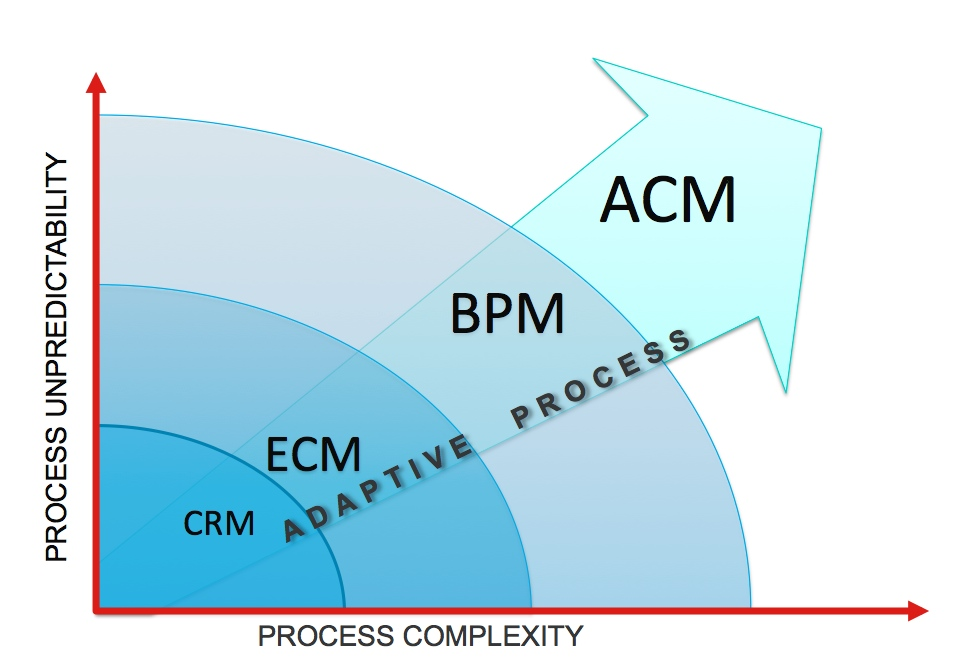
\includegraphics[width=20em]{gfx/acm-reasoning}
	\caption{https://acmisis.wordpress.com/what-is-adaptive-case-management-acm/}
	\label{fig:why-acm}
\end{figure}

\section{Predictive Modeling}
\subsection{Subsequence Mining}

\section{Predictive Modeling}
\subsection{Knowledge Discovery in Databases}
\begin{figure}
	\centering
	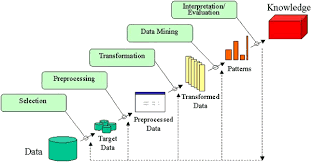
\includegraphics[width=20em]{gfx/kdd_process}
	\caption{The process for \textit{Knowledge Discovery in Databases}}
	\label{fig:kdd_process}
\end{figure}
Predictive analytics is a lot about model training, and the rough outline of necessary steps necessary to train a model is listed here:
\begin{enumerate}
	\item Determine the \textit{target} variable, it is the variable that is supposed to be predicted
	\item Preprocess the dataset. This can mean introducing one-hot encodings, normalized values, but also basic data quality assurance such as null value elimination. Feature engineering can also happen at this step.
	\item Partition the dataset into two parts. One part is set aside for model performance verification, as there the actual target variable value is known. This is commonly referred to as the \textit{test set}, while the remainder is called the \textit{training set}.
	\item Train the model on the training set. Models are trained multiple times with different hyper-parameters to find the optimum configuration with respect to prediction accuracy on the test set. Hyper-parameters are model-specific values such as cutoff-thresholds that have impact on model performance.
\end{enumerate}

\subsection{Language Modeling}
\subsubsection{Sequence-to-Sequence prediction}
\subsubsection{Sequence-to-word prediction}

\subsection{Popular feature engineering techniques}
\subsubsection{Sliding Window}
\subsubsection{N-gram}
\subsubsection{Bag-Of-Words}
\subsubsection{Learned features, word2vec}
Strictly piecewise\\
subsequences, embedding
PrefixSpan

\subsection{Neural networks}
\subsubsection{RNN}
\subsubsection{LSTM memory}
\chapter{Related Work}\label{chap:related-work}

\cleanchapterquote{A picture is worth a thousand words. An interface is worth a thousand pictures.}{Ben Shneiderman}{(Professor for Computer Science)}


Hauder et al. mention numerous research challenges in the domain of ACM, among them an active support system for knowledge workers \cite{hauder2014}.
The need for such a system is emphasized by Francescomarino et al. in their literature review, where it has been found that few prediction approaches target the next activity \cite{francescomarino2018}.

An example for how such a system might look like is given by Huber, who has developed a next-step recommendation system serving different case goals.
The system is prototypically implemented into CoCaMa\footnote{CoCaMa is an abbreviation for a project called Collaborative Case Management, which appears to be retired: \url{http://archive.li/uZFnN}}, a prototypical case management application. The system has been evaluated with 25 hand-made case logs.

Building upon each other are the works by Evermann et al. \cite{evermann2016} and Schönig et al. \cite{schoenig2018}.
Evermann et al. have successfully demonstrated the good performance of long-short-term memory (LSTM) neural networks in predicting the next activity.
Their approach did not take into account specific case data attributes however.
How making use of this contextual information can improve the prediction accuracy even more, has been shown by Schönig et al. \cite{schoenig2018}.
Furthermore Schönig et al. have explored data preparation methods for supporting the model during learning.

Similarly, Polato et al. make use of environmental information in their work for improving the prediction of the remaining time of business process instances \cite{polato2014}.

Metzger et al. predict run-time of a case by comparing and combining different prediction models into a model ensemble.
Then, the members of the ensemble are selected based on their predictive performance measures.
This allows taking into account costs of false predictions \cite{metzger2015}.

Francescomarino et al. have performed clustering in the preprocessing phase of model training and prediction.
Having clustered the training data, one model was created and trained for each cluster.
For obtaining a prediction, the optimal cluster for a new data item is found from which the corresponding model is selected.
This approach was evaluated on the accuracy of predicate fulfillment with two different clustering methods (k-means and DBSCAN) and two different prediction models (decision trees and random forests) \cite{francescomarino2015}.
A further evaluation criteria was \textit{earliness}, i.e. at which point in time the correct result could be determined.

\todo[inline]{SPICE competition submissions}
\todo[inline]{LSTM application on sequences}
\todo[inline]{LSTM application on sequences}
\todo[inline]{PrefixSpan, Strictly-Piecewise features...}

\chapter{Contribution}\label{sec:contribution}

\cleanchapterquote{Innovation distinguishes between a leader and a follower.}{Steve Jobs}{(CEO Apple Inc.)}

\section{sliding window with data}
\subsection{NULL Values}
\subsection{Staggering}

\section{sliding window with subsequence information}
\subsection{sliding window with data and prefixspan mined features}
\subsection{strictly piecewise features}




\chapter{Evaluation}\label{sec:evaluation}

\cleanchapterquote{Users do not care about what is inside the box, as long as the box does what they need done.}{Jef Raskin}{about Human Computer Interfaces}

\section{Implementation}

\section{Test setup}

\section{Evaluation criteria}

\section{Evaluation results}

\section{Result discussion}
% !TEX root = ../thesis-example.tex
%
\chapter{Conclusion}
\label{sec:conclusion}

\section{Future Work}
\label{sec:conclusion:future-work}

\section{Verdict}
\label{sec:conclusion:verdict}


\cleardoublepage

% --------------------------
% Back matter
% --------------------------
{%
\setstretch{1.1}
\renewcommand{\bibfont}{\normalfont\small}
\setlength{\biblabelsep}{0pt}
\setlength{\bibitemsep}{0.5\baselineskip plus 0.5\baselineskip}
\printbibliography[nottype=online]
\printbibliography[heading=subbibliography,title={Webseiten},type=online,prefixnumbers={@}]
}
\cleardoublepage

\listoffigures
\cleardoublepage

\listoftables
\cleardoublepage

% !TEX root = ../thesis-example.tex
%
\pagestyle{empty}
\hfill
\vfill
\pdfbookmark[0]{Colophon}{Colophon}
\section*{Colophon}

This thesis was typeset with \LaTeXe.
It uses the \textit{Clean Thesis} style developed by Ricardo Langner.
The design of the \textit{Clean Thesis} style is inspired by user guide documents from Apple Inc.

Download the \textit{Clean Thesis} style at \url{http://cleanthesis.der-ric.de/}.

\cleardoublepage

% !TEX root = ../thesis-example.tex
%
%************************************************
% Declaration
%************************************************
\pdfbookmark[0]{Declaration}{Declaration}
\chapter*{Declaration}
\label{sec:declaration}
\thispagestyle{empty}

You can put your declaration here, to declare that you have completed your work solely and only with the help of the references you mentioned.

\bigskip

\noindent\textit{\thesisUniversityCity, \thesisDate}

\smallskip

\begin{flushright}
	\begin{minipage}{5cm}
		\rule{\textwidth}{1pt}
		\centering\thesisName
	\end{minipage}
\end{flushright}

%*****************************************
%*****************************************

\clearpage
\newpage
\mbox{}

% **************************************************
% End of Document CONTENT
% **************************************************
\end{document}
